\documentclass[titlepage]{article}
\usepackage[bottom=3cm, right=3cm, left=3cm, top=3cm]{geometry}
\usepackage {graphicx}
\usepackage{caption}
%opening
\title{%
	Practical Machine Learning\\
	
	\vspace*{2em}
	\LARGE Exercise 2 \\
	Spring 2024}
\author{Lisa Stafford}
\date{February 14, 2024}

\begin{document}

\maketitle

\captionsetup{
	format = plain,
	font = footnotesize,
	labelfont = sc
}

\section*{Abstract}
Data preprocessing is a method utilized in the machine learning pipeline to transform raw data into an understandable format by performing  analysis, filtering, transformation, and encoding of data so that machine learning algorithms can understand and work with the data as appropriate.  This is a very important step in machine learning because it does a quality check upon the data, and determines accuracy, completeness, consistency, and how easily interpreted the data is.  If this is not done correctly, the quality and performance of the machine learning model suffers as a consequence.  The primary steps in preprocessing are the initial data collection, cleaning, integration, transformation, reduction, discretizing, normalization, standardization, feature selection, and representation.  In this exercise we seek to perform all preprocessing steps and determine how they effect the overall performance of a static, pre-selected machine learning model architecture while making dynamic changes to preprocessing actions and evaluating the compared performance.   

\section*{Background and Introduction}
In order to learn and determine in which situations data preprocessing can be effective, and how, we analyze two different datasets - a tumor dataset originally obtained from University Medical Center, Institute of Oncology in Yugoslavia  \cite{dataset1} and a wine data set obtained from the University of Irvine \cite{dataset2}.  We use a consistent machine learning model for each dataset (in this case using the scikit-learn decision tree library) and then determining what (if any) preprocessing methodologies are most effective in preparing our two datasets for machine learning by evaluating the overall performance of the models after taking these datasets in standard and consistent ways, and modifying them using different preprocessing techniques, then evaluating performance of the model per each preprocessing step/activity.  

\section*{Results of the Analysis: Wine Datasets}
Our Wine Dataset is actually comprised of two different wine subsets of data.  While both are related to variants of \cite{dataset2} "Portuguese Vhinho Verde wine" the data is actually split in two subsets - one red subset and one white subset.  Each subset contains 11 features and 1 label for wine quality.   All features are continuous float values.  Within the model the "wine quality" labels are recognized as discrete categorical integer values ranging from 3 to 9 for the white wines, and 3 and 8 for the red wines.  White wine contains a total of 4898 total data instances, while red wine has a total of 1598 data instances as shown in the following table images. Figure 1 (left) displays feature values, statistics, and total instances for white wine, while Figure 1 (right) displays feature values, statistics and total instances available for red wine.

\begin{figure}
	\centering
	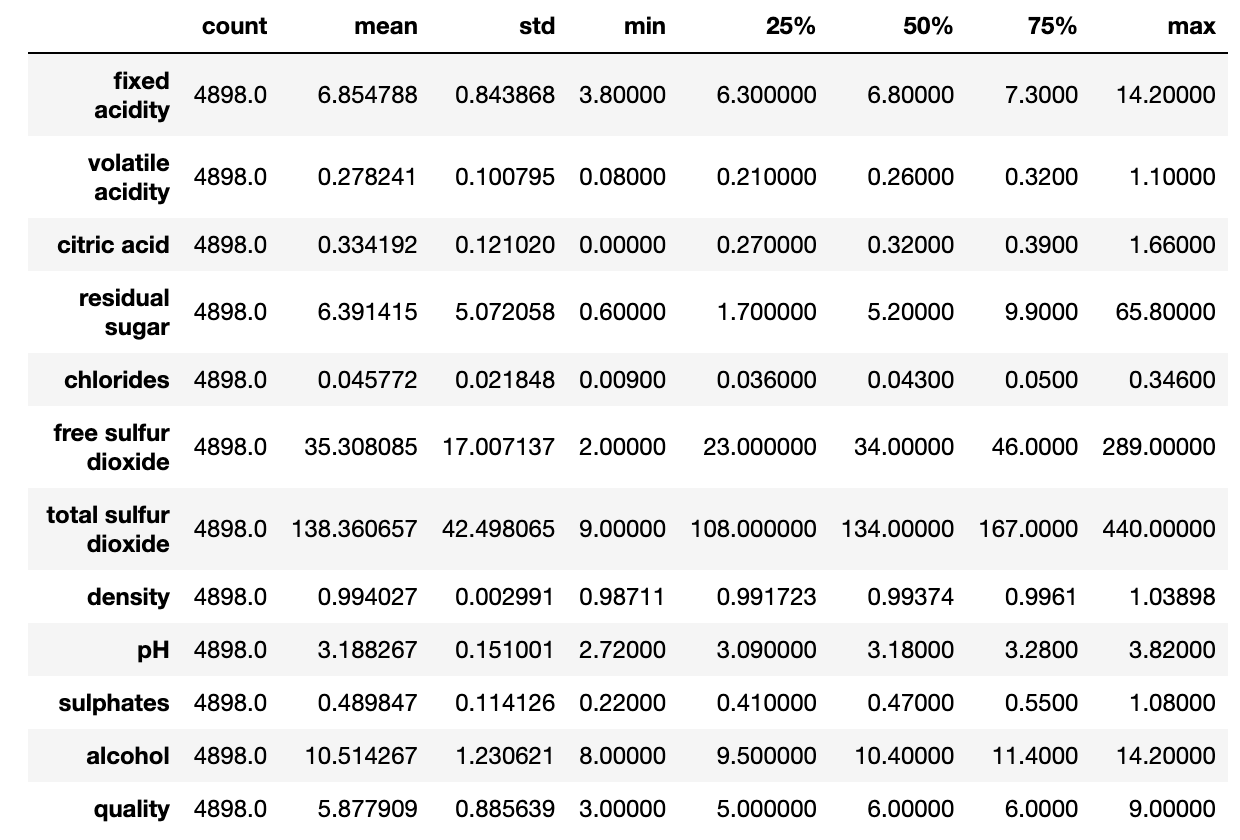
\includegraphics[width=.45\textwidth]{img/whitestats.png}
	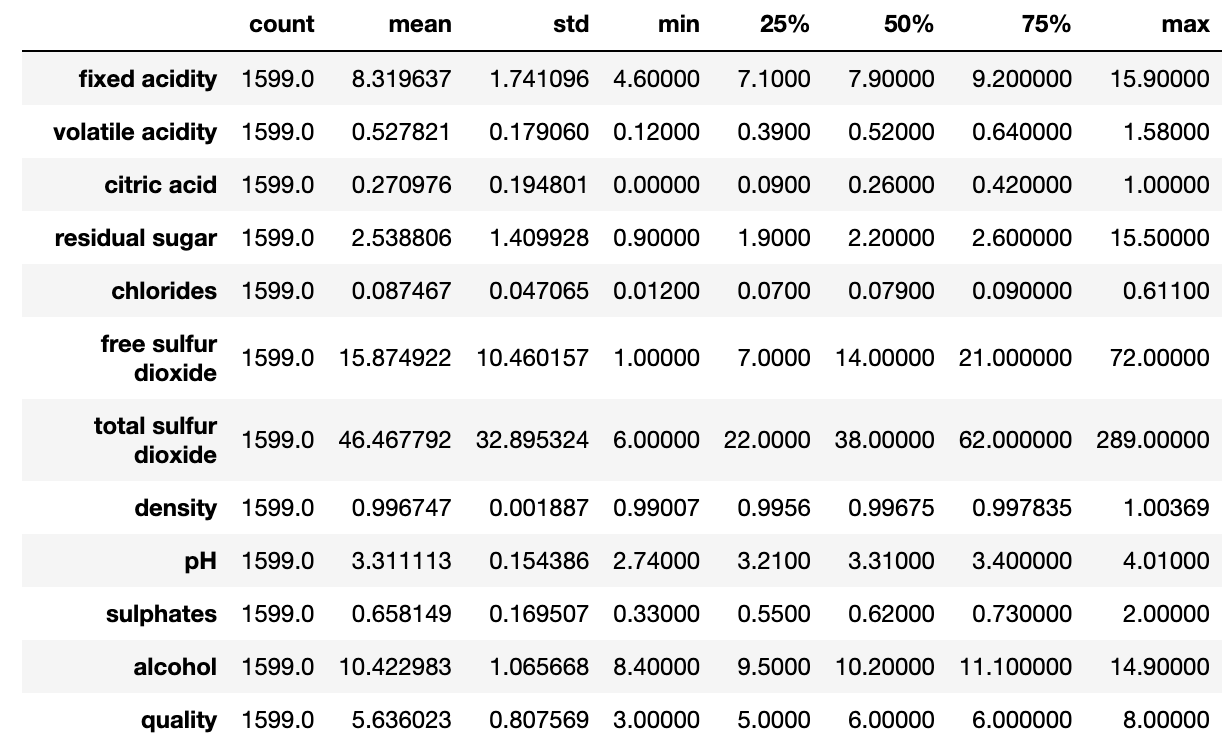
\includegraphics[width=.45\textwidth]{img/redstats.png}
	\caption{ Wine Datasets:  White on Left, Red on Right}
\end{figure}


\noindent Data for both red and white wine datasets is somewhat "pre-cleaned".   The feature values are all continuous and both red and white datasets contain no missing data values.  However it should be noted that these features are not evenly distributed.  The data values are somewhat bell-shaped with a larger number of data instances with labels closer to the mean.  As described on the dataset website \cite{dataset2} both "dataset... classes are ordered and []unbalanced] so there are many more normal wines than excellent or poor ones.... [also], both datasets have 11 physiochemical features... and a sensory output label, ('quality')".  The two figures below this text are histograms corresponding to white and red [Figure 3] wine quality and distributions.  

\begin{figure}
	\centering
	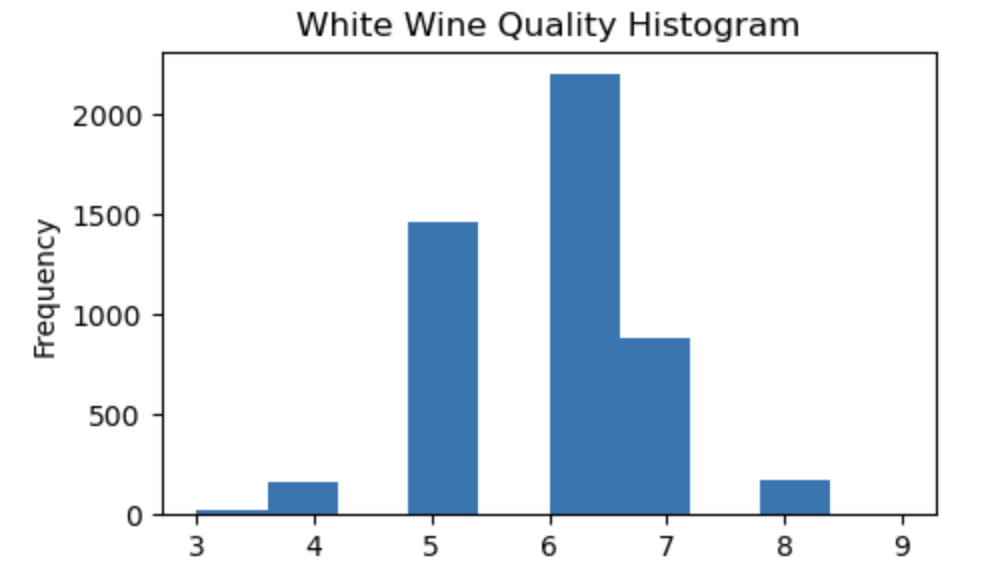
\includegraphics[width=.4\textwidth]{img/whitehistogram.png}
	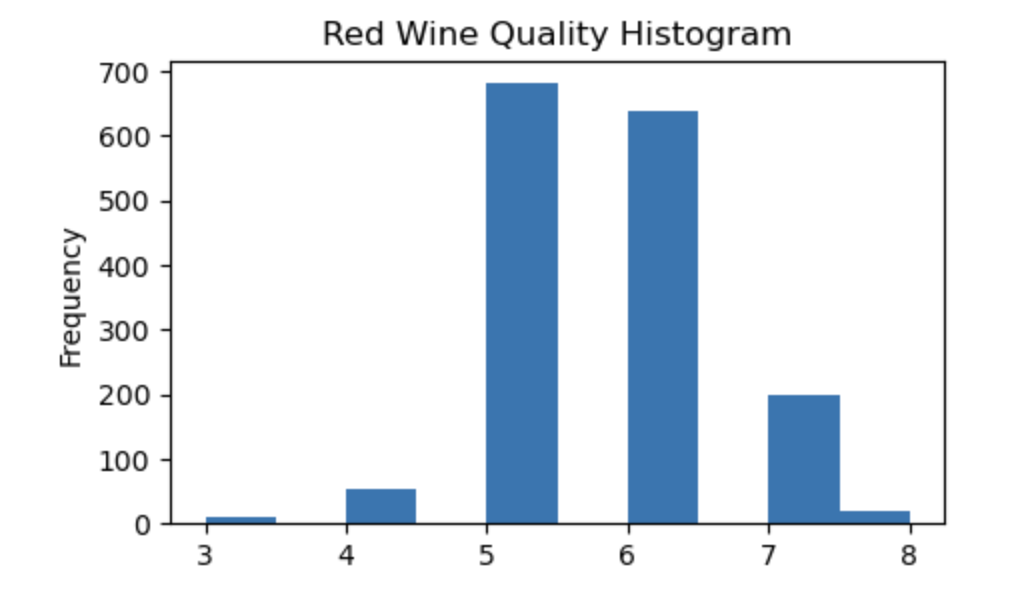
\includegraphics[width=.4\textwidth]{img/redhistogram.png}
	\caption{Wine Quality Distributions: with White on Left, Red on right}
\end{figure}


\noindent With what we know about our wine data, this we can already provide information about our future machine learning model.  Preprocessing will include some method of data normalization, and we will be doing supervised training on the data to predict wine quality. 

\noindent If we simply perform machine learning on the dataset without any preprocessing we can obtain a base case for model performance on the dataset.  A confusion matrix on the left of Figure 4 shows our first run of such a model on the white wine data, which performed with an accuracy score of 57.86\%:    

\begin{figure}
	\centering
	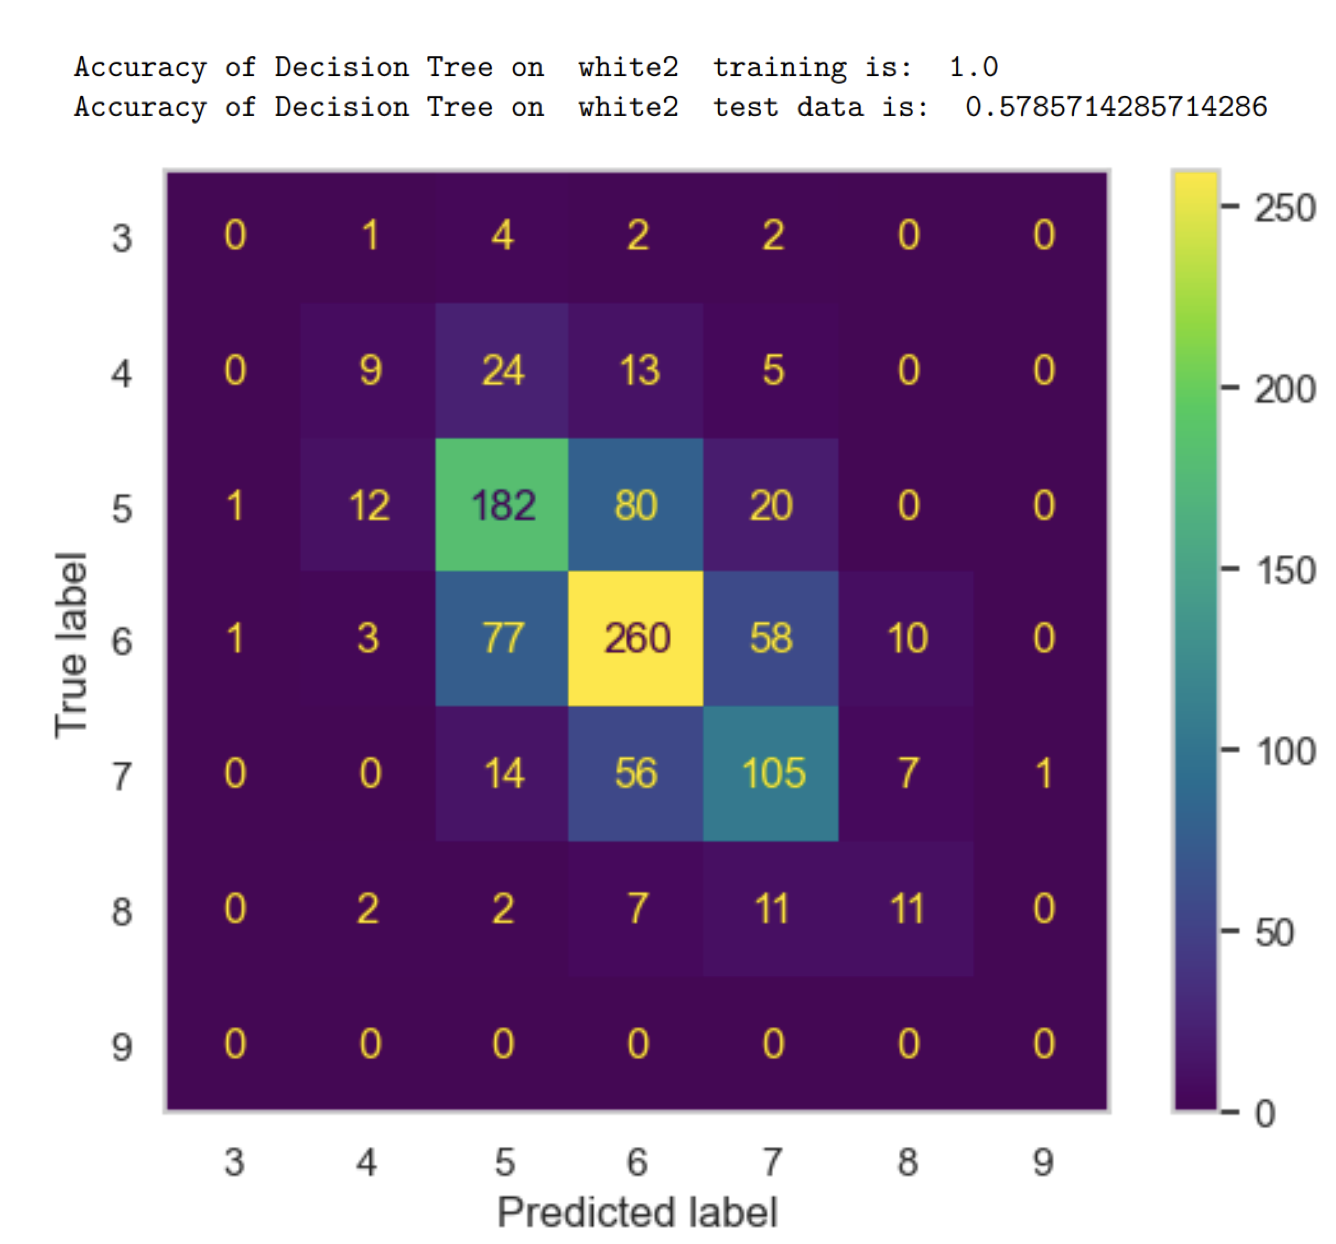
\includegraphics[width=.36\textwidth]{img/whitematrix.png}
	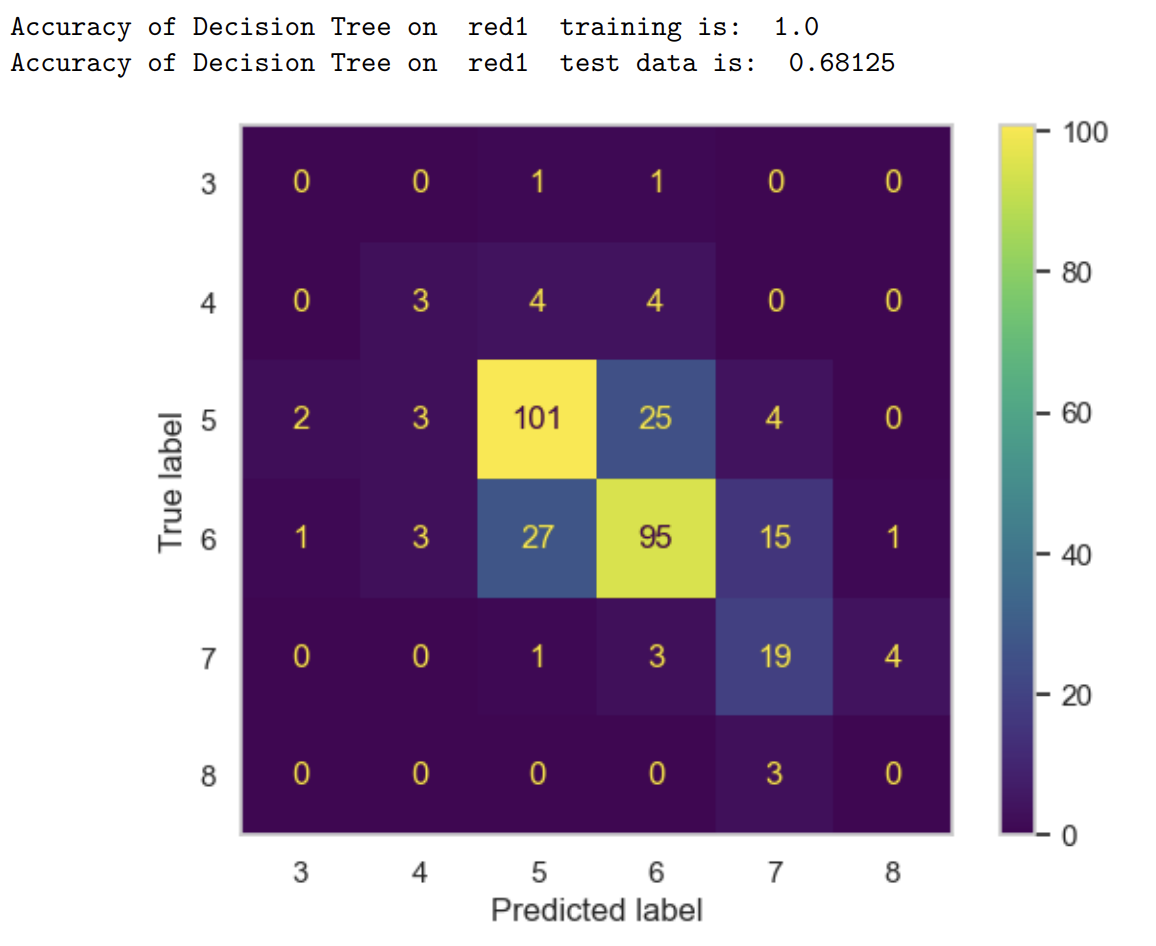
\includegraphics[width=.4\textwidth]{img/redmatrix.png}
	\caption{Wine Test Performance Base Case: White on Left, Red on Right}
\end{figure}


\noindent Performing base case machine learning on red wine dataset performed similarly, with an accuracy score of 68.125 \% as shown on the right matrix in the figure [Figure 4].  Over 5 iterations of both the white and red wine datasets, average accuracy was 57.61\% for white wines and  67.25\% for red wines.  After performing an initial normalization on the feature data for both the red and white wine datasets, accuracy after 5 iterations seemed to drop noticeably for the red wine model 61.3\% while remaining relatively consistent for the white wine model 57.5\%.  I would assume this is likely because of the larger size of the white wine dataset, but cannot say for sure why this is the case without additional investigation.

\noindent As we iterate through possible data processing actions, from the base case since we do not have to deal with null data or missing values, we perform the following  data cleanup tasks:
\begin{enumerate}
	\item Normalize features
	\item Perform StandardizedScaling on Features
	\item Determine which features have most value within the dataset to determine quality, and make those "matter" more.
\end{enumerate}

\noindent The resulting performance of a model trained on different data scaling and transforming is shown below for both the red and white datasets, when compared to the base training:  
\subsection*{Training on Red Wine Data}
\begin{center}
	\begin{tabular}{ | c | c | c | }
		\hline
		& \textbf{Train Accuracy} & \textbf{Test Accuracy} \\ 
		\hline
		\textbf{Base Case } & 100\% & 66.93\% \\
		\textbf{Normalization} & 100\% & 60.25\% \\
		\textbf{Standard Scaling and Transform} & 100\% & 68.39\%  \\
		\hline
	\end{tabular}
\end{center}

\subsection*{Training on White Wine Data}
\begin{center}
	\begin{tabular}{ | c | c | c | }
		\hline
		& \textbf{Train Accuracy} & \textbf{Test Accuracy} \\ 
		\hline
		\textbf{Base Case} & 100\% & 57.57\% \\
		\textbf{Normalization} & 100\% & 57.12\% \\
		\textbf{Standard Scaling and Transform} & 100\% & 59.6\%  \\
		\hline
	\end{tabular}
\end{center}

As we look through the dataset we can determine several things:  
\begin{enumerate}
	\item So far normalization and scaling doesn't seem to result in much of a change to performance.  Standard Scale and Transform results in a slight change.  
	\item Histograms of both Red and White Wine label distribution suggest significantly skewed samples and unbalanced data.  A large majority of all wines are labeled with qualities 5 or 6 but minimal samples are provided for other quality classes 3, 4, 7, 8, and 9.  Some research suggests this can be corrected through resampling.  
	\item Most features also tend to be skewed towards the right. Those most skewed are Residual Sugar, Chlorides, Free Sulphur Dioxide, Total Sulphur Dioxide, and Sulphates. Such features may need to be transformed for certain model algorithms by applying transformation to improve classification performance.
	\begin{center}
		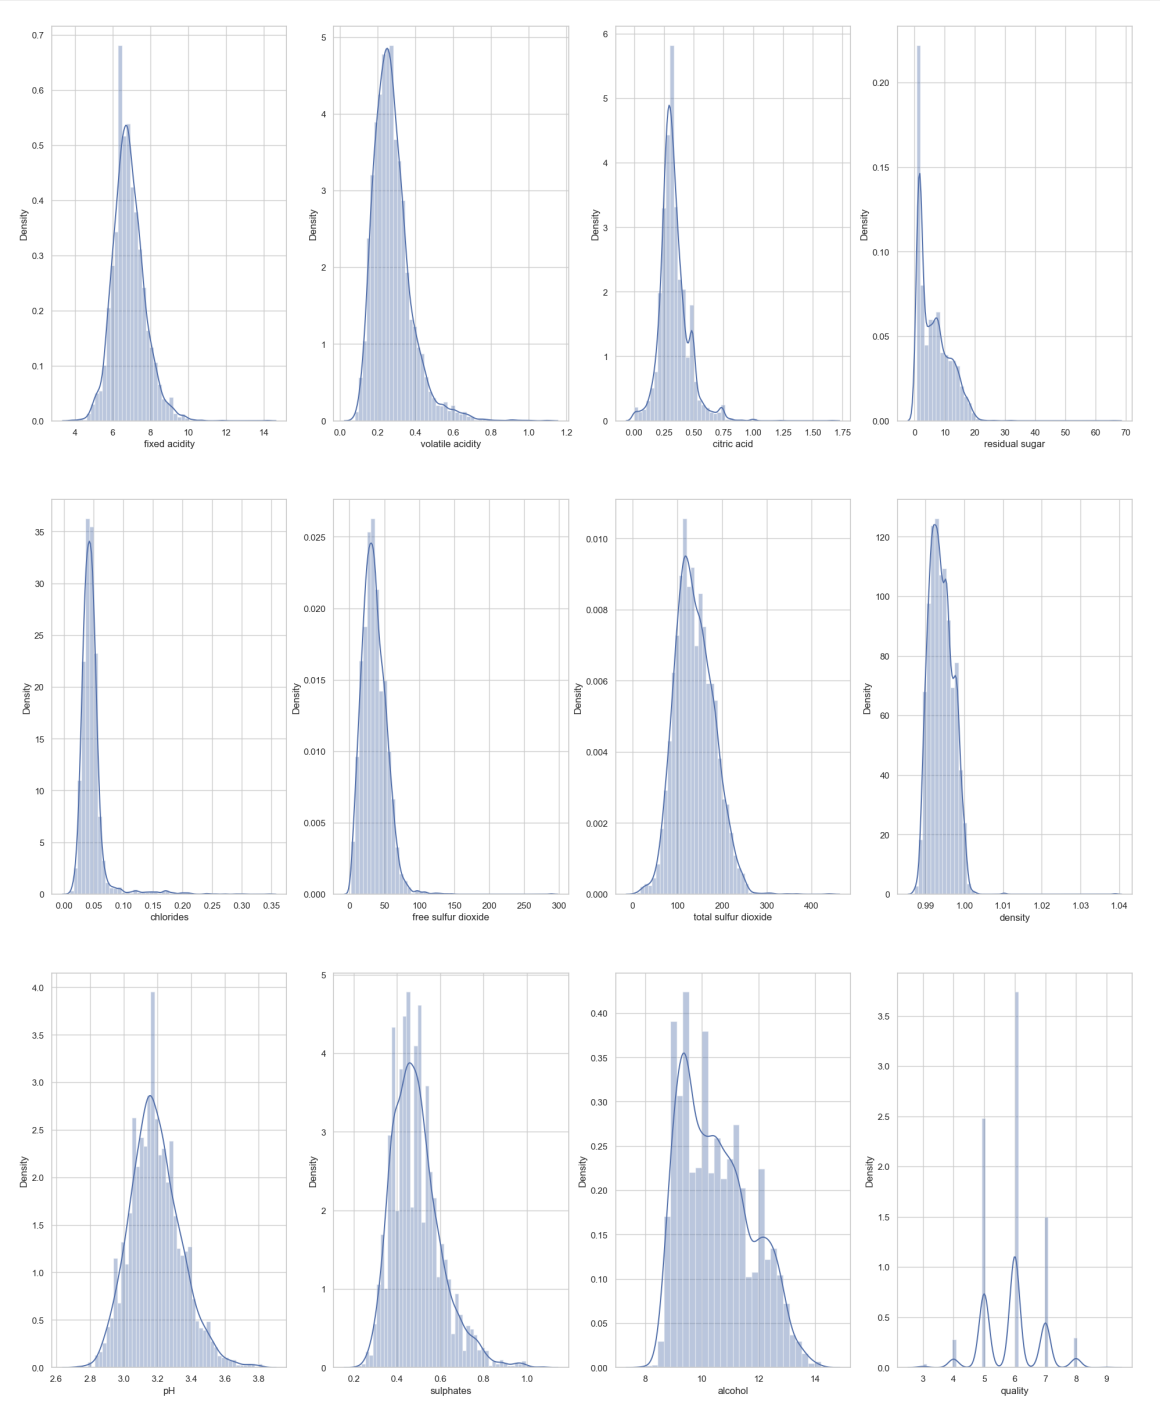
\includegraphics[width=.6\textwidth]{img/featureskews.png}
	\end{center}

\end{enumerate}

To make things a little quicker, at this point, performance evaluation is focused upon the white dataset only as that seems to have more room for improvement.  We attempt to unskew some of the features using a logrithmic transformation on certain data features.  

We perform log transformation on residual sugars, chlorides, free sulfur dioxide, total sulfur dioxide, and sulfates.  
\newline
\begin{center}
	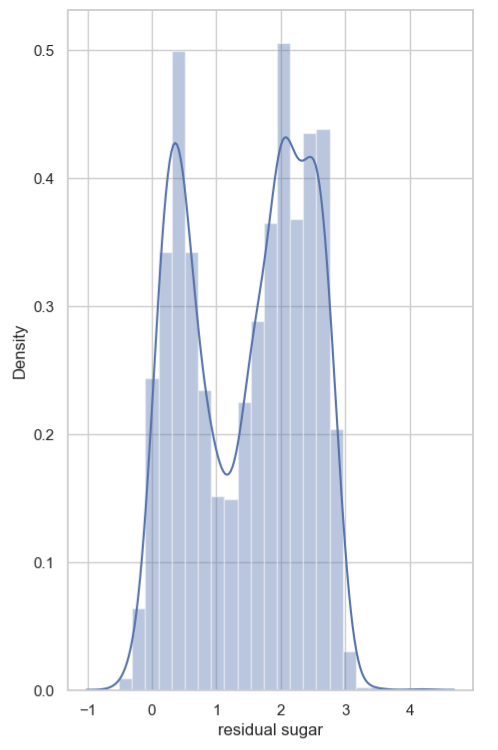
\includegraphics[width=.17\textwidth]{img/logscaledfeatures1.png}
	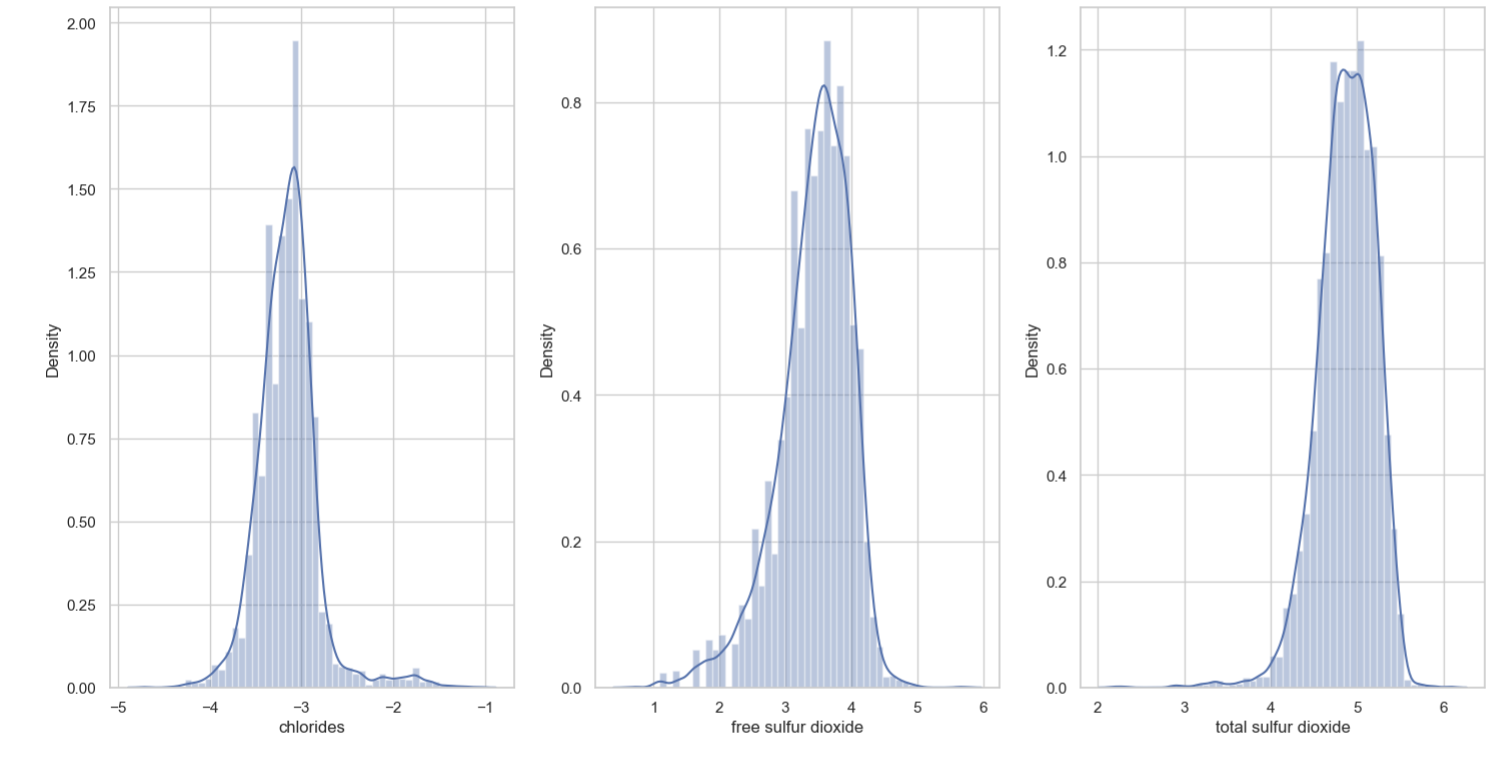
\includegraphics[width=.5\textwidth]{img/logscaledfeatures2.png}
	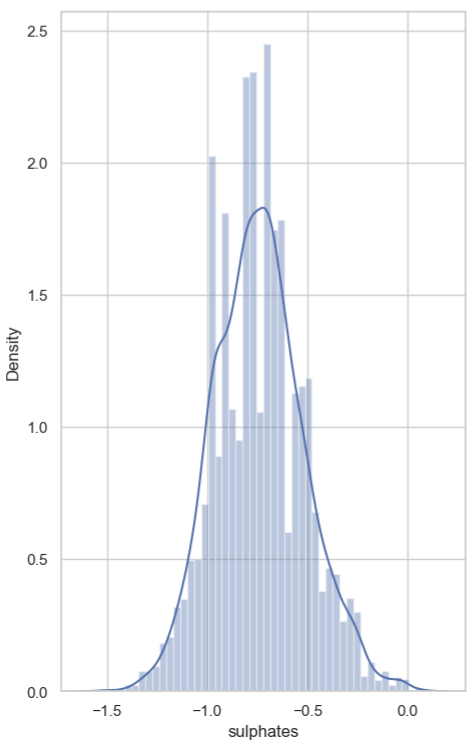
\includegraphics[width=.17\textwidth]{img/logscaledfeatures3.png}
\end{center}

Performance after log scaling specific features in the dataset does not appear to have a large effect on total performance.  The result of 5 runs is an average accuracy of 58.1\%, somewhat similar to the performance result improvement when using standard scaler transformation.

Our last attempt to improve performance is based upon trying to use resampling to provide more samples of underrepresented classifications.  Towards that end we upsample classes 3,4,7,8, and 9 using the resample library in scikitlearn resulting in a total of 1000 samples in each of those classifications, respectively.  Upon doing so, performance appears to have jumped up significantly:  
\newline
\begin{center}
	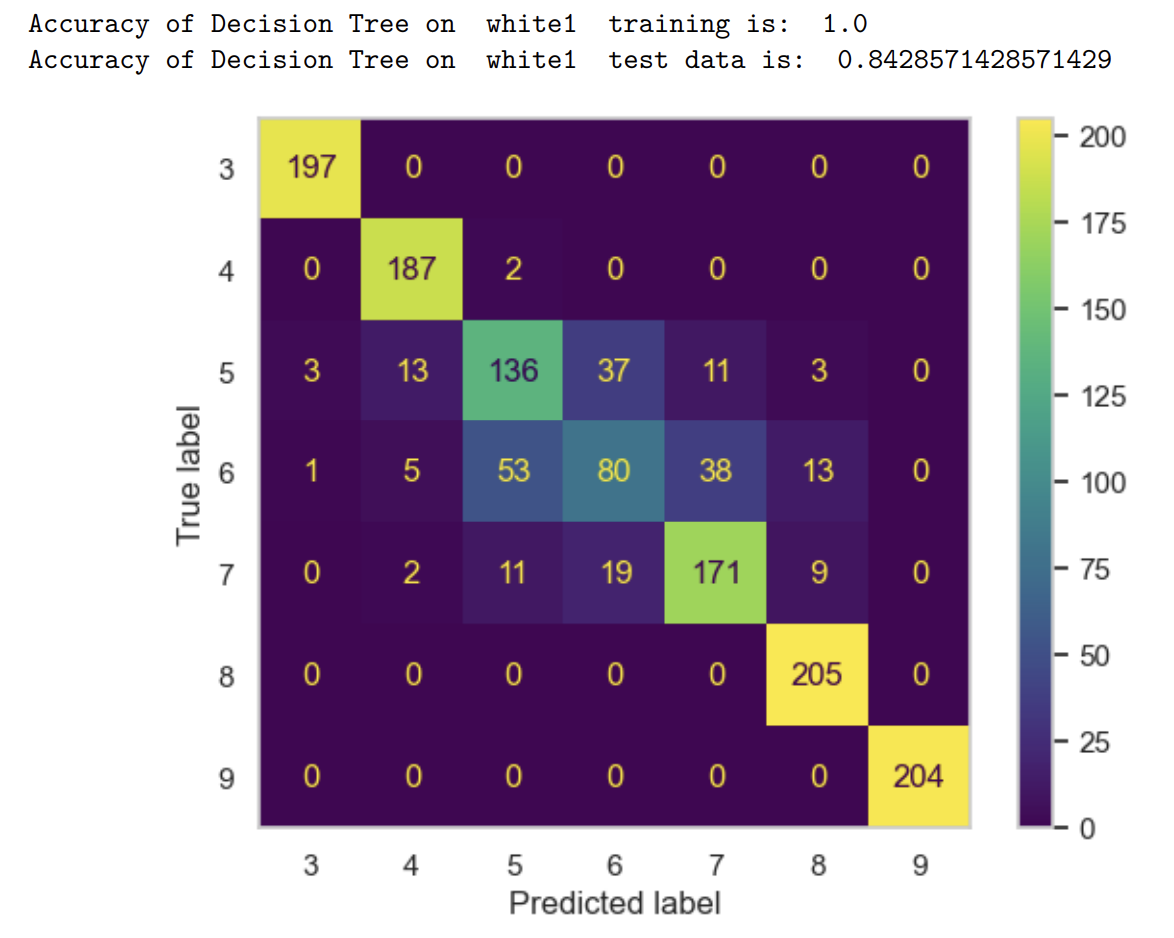
\includegraphics[width=.5\textwidth]{img/resampledmatrixwithscores.png}
\end{center}

While this initially seems like a reason for celebration, it is misleading.  Because scikitlearn's resampling library basically duplicates samples to result in more of them, those same samples are leaked from the training to the test data resulting in identical data instances and observations in both training and testing, leading to a very high number of correct predictions on under-represented classifications within the test performance.  

To correct this, we need to go back and only train the model on the resampled data, but stick with the un-resampled data in testing.  When we do that, we notice that the performance has actually dropped slightly:  
\newline
\begin{center}
	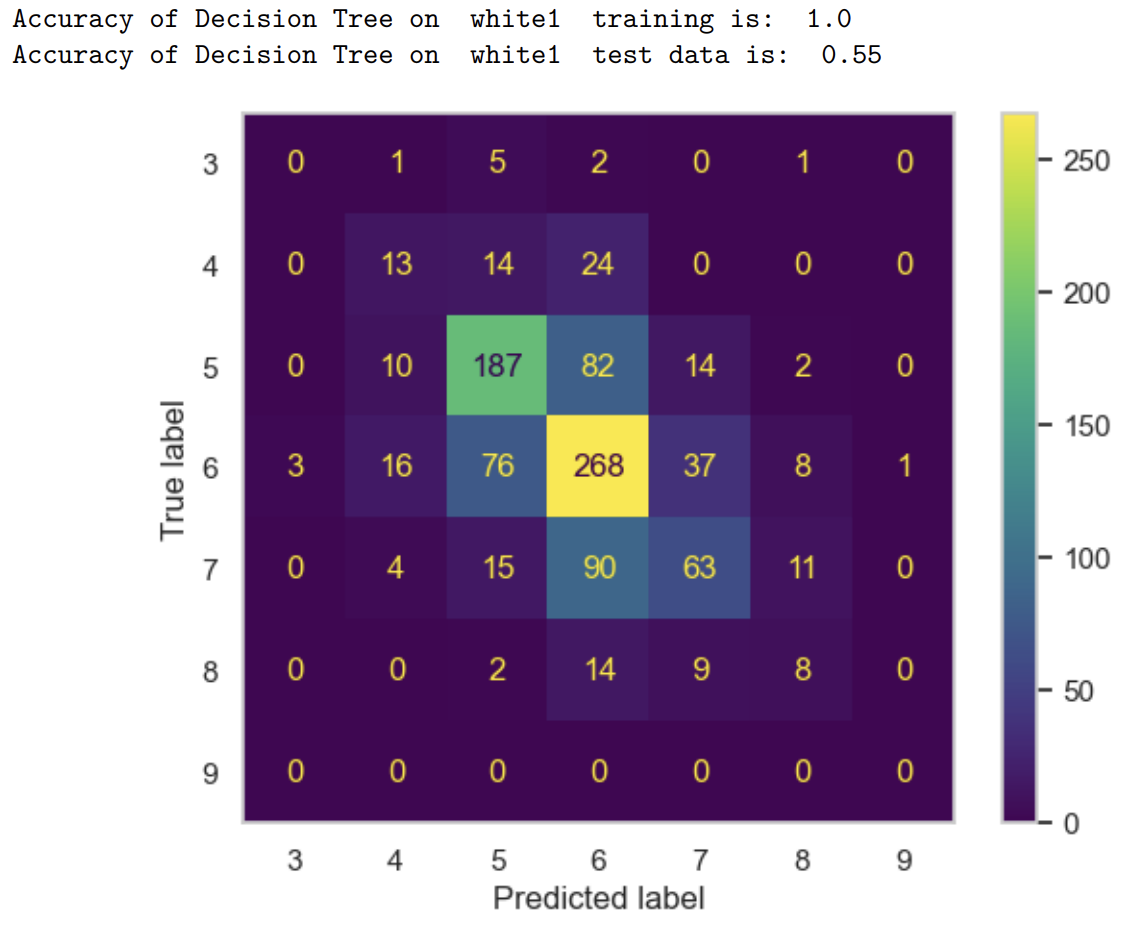
\includegraphics[width=.5\textwidth]{img/resamplematrixnodataleak.png}
\end{center}

This is suspected because the trained model no longer sees outlier values as outliers and would predict them more often than otherwise because the model doesn't account for their less likely occurrence in overall prediction.  


\section*{Results of the Analysis: Tumor Dataset}
Our Tumor dataset was obtained from the openml website \cite{dataset1} and consists of 17 total features and a single binary label that is either positive or negative listed in the dataset as "N" or "P".  There are 339 instances in the data.  Additionally, the data repository contains some initial analysis on the data and some of those images can be viewed within this document. Several features contain missing data and 2 features ('degree-of-diffe' and 'histologic-type') contain a large number of missing values, 155 and 67 respectively. These missing values show up in the data as '?" of type string/object and need to be changed so that they are recognized as null values within the set.  A large number of instances also have individual instances contain some form of missing value (207 of the total 339 which is significant). Therefore simply deleting any instances with missing values would significantly limit out data set and is not a suitable solution for this particular collection of data.  

\vspace{.5cm}\noindent Since the cancerdata is imported from a .arff file, it contains b' characters before every feature. To correct this, we must decode the strings in utf-8. The output/label data is listed in pandas as an object despite being titled "binaryClass". Ideally, preprocessing work would clean the data by filling in the missing data with values that didn't affect the overall model while also standardizing the data for better readability by anyone who would like to interpret the data and remove any noise caused by additional characters or improperly categorizing data types that could influence the model training.  

\vspace{.5cm}\noindent To visualize the data, we first must update all "?" values in the dataset converting them to np.nan so they are picked up by numpy \cite{numpyisnan} and other data analysis libraries.  After doing so, we can visualize the data using a Seaborn \cite{seaborn} heatmap to show missing data within the dataset in Figure 5.  

\begin{figure}
	\centering
	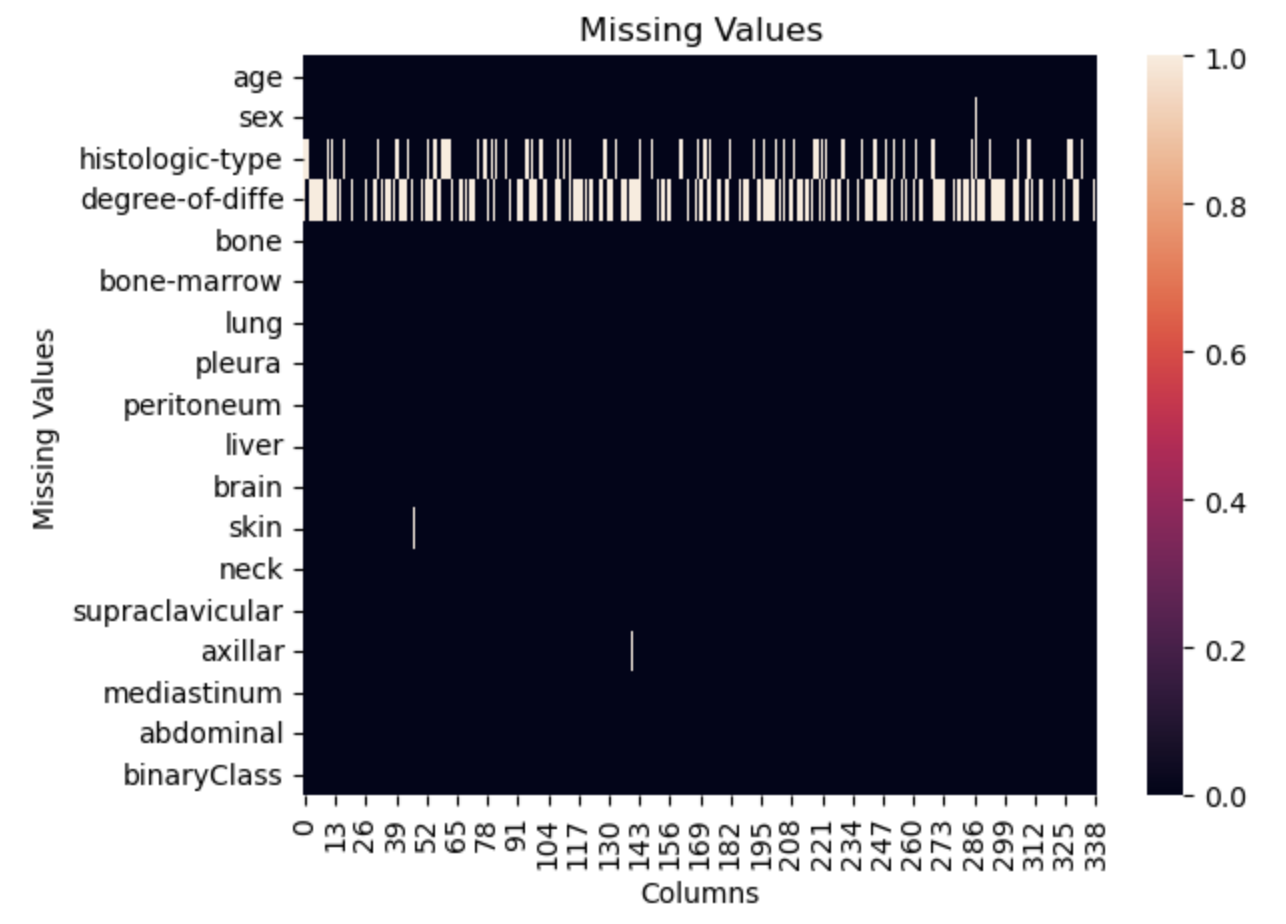
\includegraphics[width=0.65\linewidth]{img/cancerheatmap.png}
	\caption{Missing Cancer Features in Dataset}
	\label{fig:cancerheatmap}
\end{figure}

\vspace{.5cm}\noindent After viewing the missing data visually, we can note that degree-of-diffe and histologic-type values are both primary missing values.  These values in the dataset appear to be "Missing at Random" values, meaning that the missing values are conditional, dependent upon other data available within the dataset.  So the data is not missing for all observations, only those within sub-samples based upon a pattern.    First we attempt to show nullity correlation between columns and features within the dataset.  This can also be displayed visually as a heatmap in the figure 6.

\begin{figure}
	\centering
	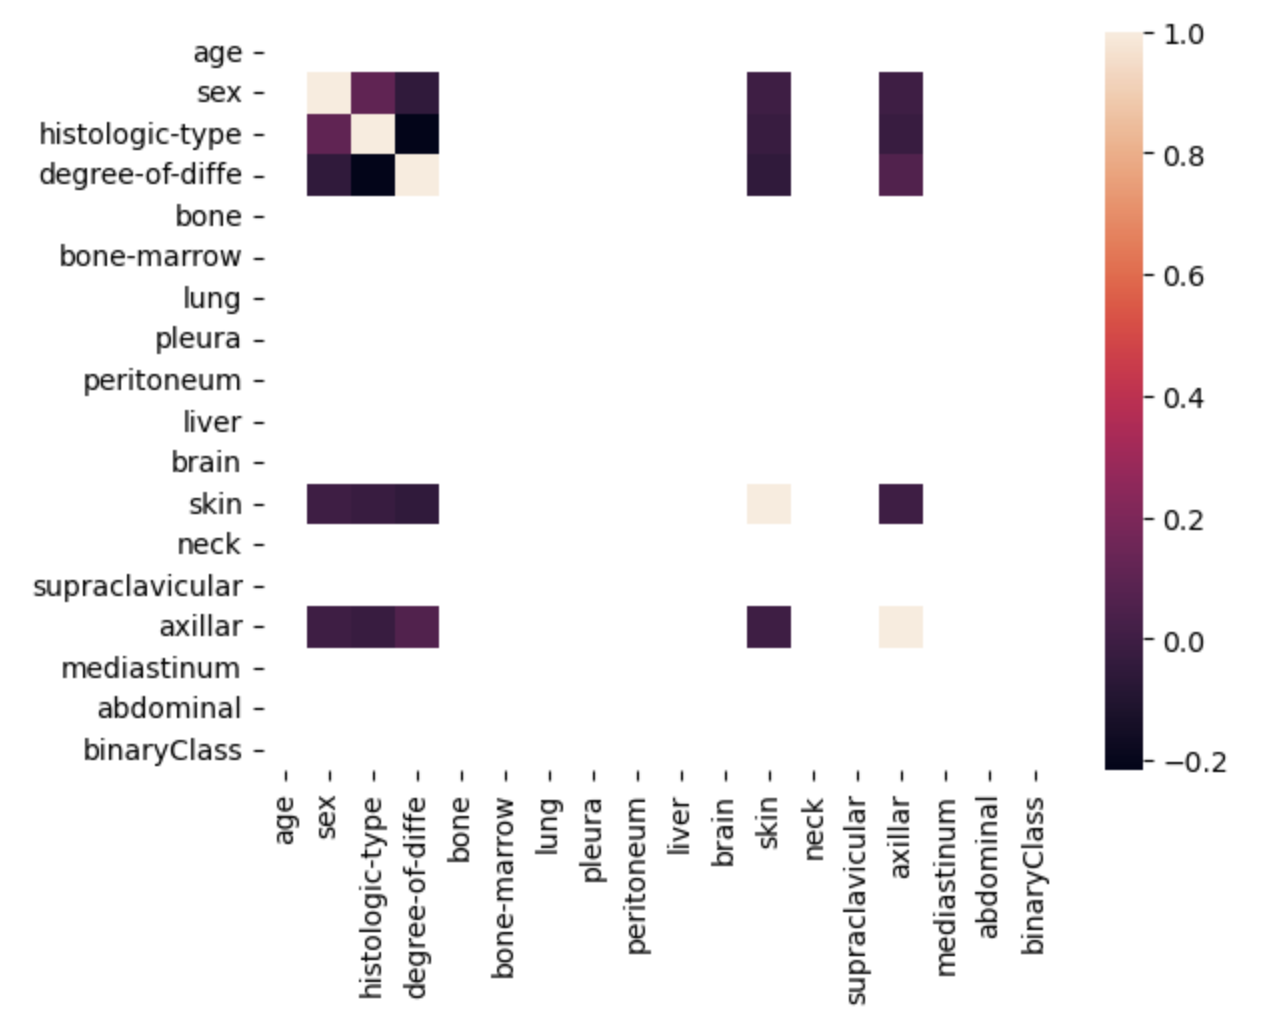
\includegraphics[width=0.65\linewidth]{img/missingheatmap.png}
	\caption{Missing Dataset Correlation Heatmap}
	\label{fig:missingheatmap}
\end{figure}

To preprocess this data further - performing normalization and encoding all classes, we make use of scikit-learn's \cite{scikitlearn} prepackaged encoder libraries, $LabelEncoder()$, $TargetEncoder()$, and $OneHotEncoder()$. Average accuracy of model performance after normalizing and transforming data using each of these encoders is displayed in the table below:  
\begin{center}
\begin{tabular}{ | c | c | c | }
	\hline
	  & \textbf{Train Accuracy} & \textbf{Test Accuracy} \\ 
	  \hline
	\textbf{Label Encoder} & 99.25\% & 81.0\% \\
	 \textbf{Target Encoder} & 99.999\% & 76.47\% \\
	 \textbf{One Hot Encoder} & 99.26\% & 82.353\%  \\
	\hline
\end{tabular}
\end{center}


\section*{Code}
Code is provided in 3 jupyter notebooks.  One specifically for wine data, one for cancer/tumor data, and the last an exercise2 notebook which consolidates collected information from both datasets.   Code and all relevant files and information related to the project may be found at the following repository:  https://github.com/COSC5557/exploratory-data-analysis-lrstafford 

\begin{thebibliography}{9}
		\bibitem{dataset1} I. Kononenko, B. Cestnik,  Primary Tumor Domain, University Medical Centre, Institute of Oncology, Jozef Stefan Institute, Ljubljana Yugoslavia, (1988). Obtained from https://www.openml.org/search?type=data\&sort=runs\&id=171
		\bibitem{dataset2} A. Asuncion, D. Newman, UCI Machine Learning Repository, University of California, Irvine  (2007).  Obtained from https://archive-beta.ics.uci.edu/dataset/186/wine+quality. 
		\bibitem{numpyisnan} C. Harris, K. Millman, S. van der Walt,  Array programming with NumPy. Nature 585, 357–362 (2020). DOI: 10.1038/s41586-020-2649-2.  https://numpy.org/doc/stable/reference/generated/numpy.isnan.html
		\bibitem{seaborn} M. Waskom, (2021). seaborn: statistical data visualization. Journal of Open Source Software, 6(60), 3021, https://doi.org/10.21105/joss.03021.
		\bibitem{scikitlearn}Scikit-learn: Machine Learning in Python, Pedregosa et al., JMLR 12, pp. 2825-2830, 2011. 
\end{thebibliography}

\end{document}
